\documentclass[10pt, letterpaper]{article}

% Language setting
% Replace `english' with e.g. `spanish' to change the document language
\usepackage[english]{babel}

% Set page size and margins
% Replace `letterpaper' with`a4paper' for UK/EU standard size
\usepackage[letterpaper,top=2cm,bottom=2cm,left=3cm,right=3cm,marginparwidth=1.75cm]{geometry}

% Useful packages



\usepackage{fancyvrb}
\usepackage{fancyhdr, lastpage}
\pagestyle{fancy}
\lhead{Parker Levesque}
\rhead{CTA200}
\cfoot{Page \thepage\ of \pageref{LastPage}}

\usepackage[Glenn]{fncychap}
%Options: Sonny, Lenny, Glenn, Conny, Rejne,
%Bjarne, Bjornstrup

\usepackage{xcolor}

\usepackage{tikz, tcolorbox}

\usepackage{physics}
\usepackage{amsmath,amsthm,amssymb}
\usepackage[dvips,letterpaper,margin=1.1in,bottom=0.7in]{geometry}
\usepackage{graphicx}
\usepackage{hyperref}
\hypersetup{
    colorlinks=true,
    linkcolor=blue,
    urlcolor=red,
    pdftitle={Template}
    }
\usepackage{enumitem}
\usepackage{charter}
\usepackage{tabstackengine}
\usepackage{siunitx}
\usepackage[font=small,labelfont=bf]{caption}
\usepackage{mwe}
\usepackage[sorting=none]{biblatex}




\usepackage{listings}
\usepackage{subcaption}
\usepackage{wrapfig}
\usepackage{indentfirst}
\usepackage{float}
\usepackage{geometry}
\usepackage{lipsum}
\usepackage[nice]{nicefrac}
\counterwithin{figure}{section}

\captionsetup{justification=centering,margin=2cm}



\newcommand{\ds}{\displaystyle}

\title{Assignment \# 3 - CTA200}
\author{Parker Levesque \\ parker.levesque@mail.utoronto.ca}

\date{May, 2021}

\begin{document}



\maketitle

\newpage


\section{Question 1}

We wish to grab each point in the complex plane $\left( c = x + iy \right)$, and iterate the equation:

\begin{align}
    z_{i+1} = z_{i} + c \label{eq:1}
\end{align}

given the initial value $z_0 = 0$. The domain of interest is given by $-2 < x,y < 2$.

If the square modulus of a complex number $\left( |z|^2 = Re(z)^2 + Im(z)^2 \right)$ in our domain goes off to infinity, we first set its value to zero, otherwise the converging points are set to one. The binary map is visualized in Figure \ref{fig:m1}.

\begin{figure}[H]
    \hspace*{-5mm}
        \centering
        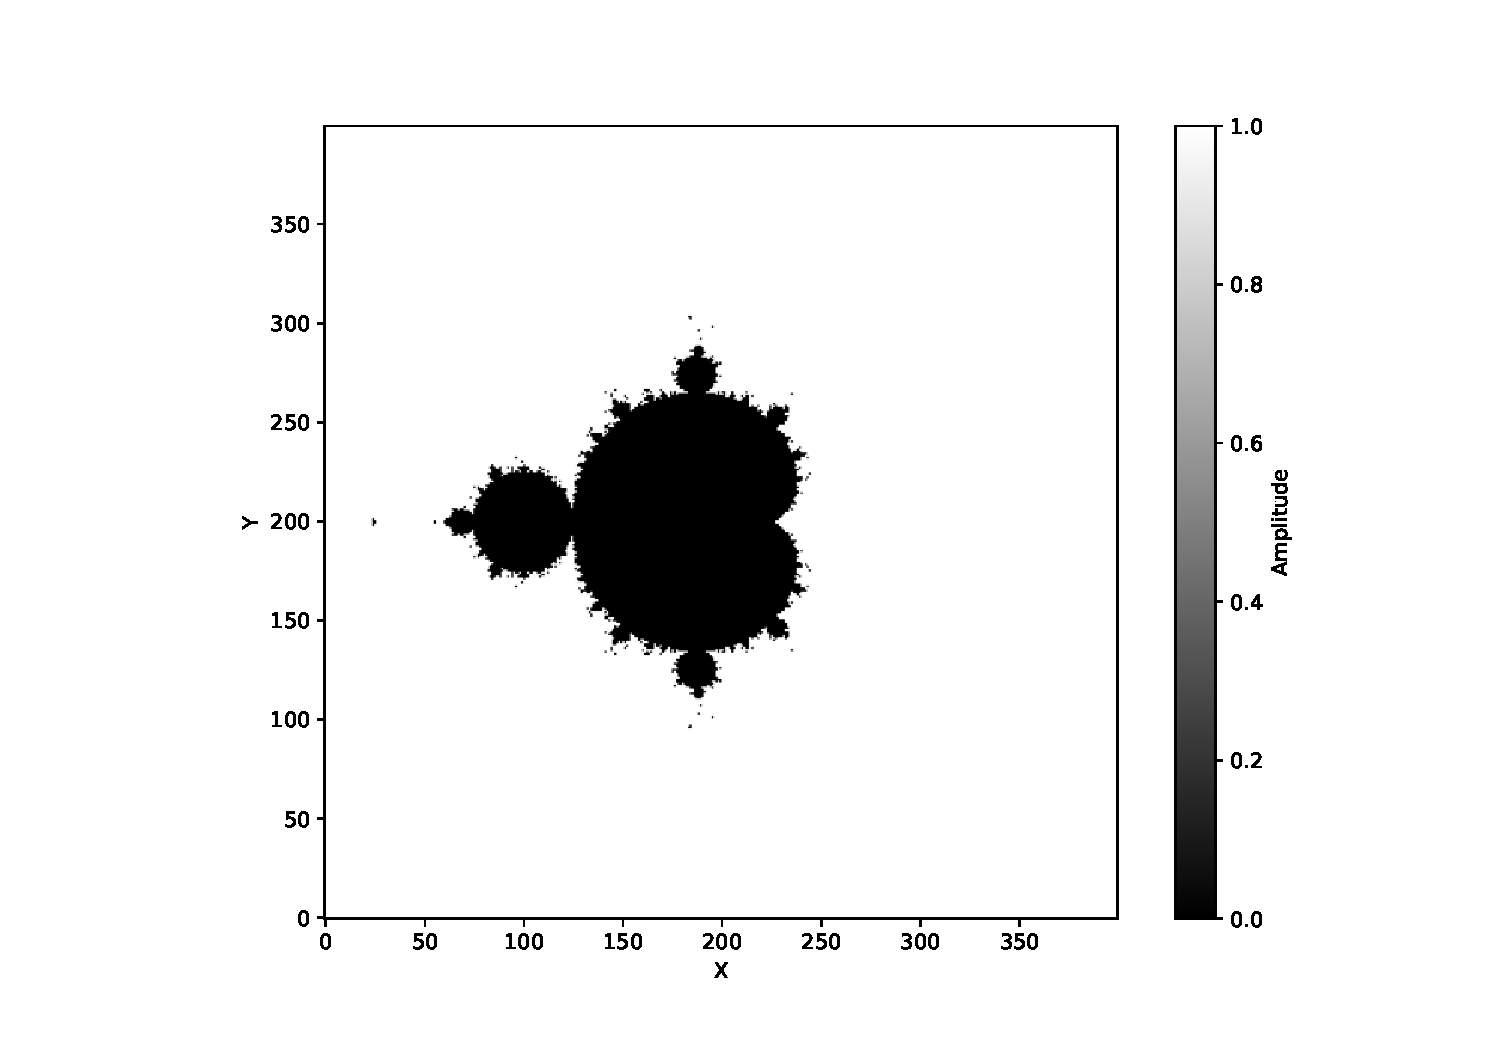
\includegraphics[width =\textwidth]{mandel1.pdf}
        %\vspace{-15mm}
        \caption{The binary plot of the diverging points contrasted by the converging points, when iterated through equation \ref{eq:1}}
        \label{fig:m1}
\end{figure}

However, we may also track the progress of each point throughout the iteration. When an initial seed is iterated through equation \ref{eq:1}, we consider a divergence to occur at step $i$, when $z_{i+i}$ appears outside of our domain of interest. So, tracking the square modulus of the point with each iteration, we may store the iteration value at which it diverges. We may visualize this map of `characteristic divergence numbers' in Figure \ref{fig:m2}, where we sample 400x400 points on the complex plane and iterate 50 times in total.

\begin{figure}[H]
    \hspace*{-5mm}
        \centering
        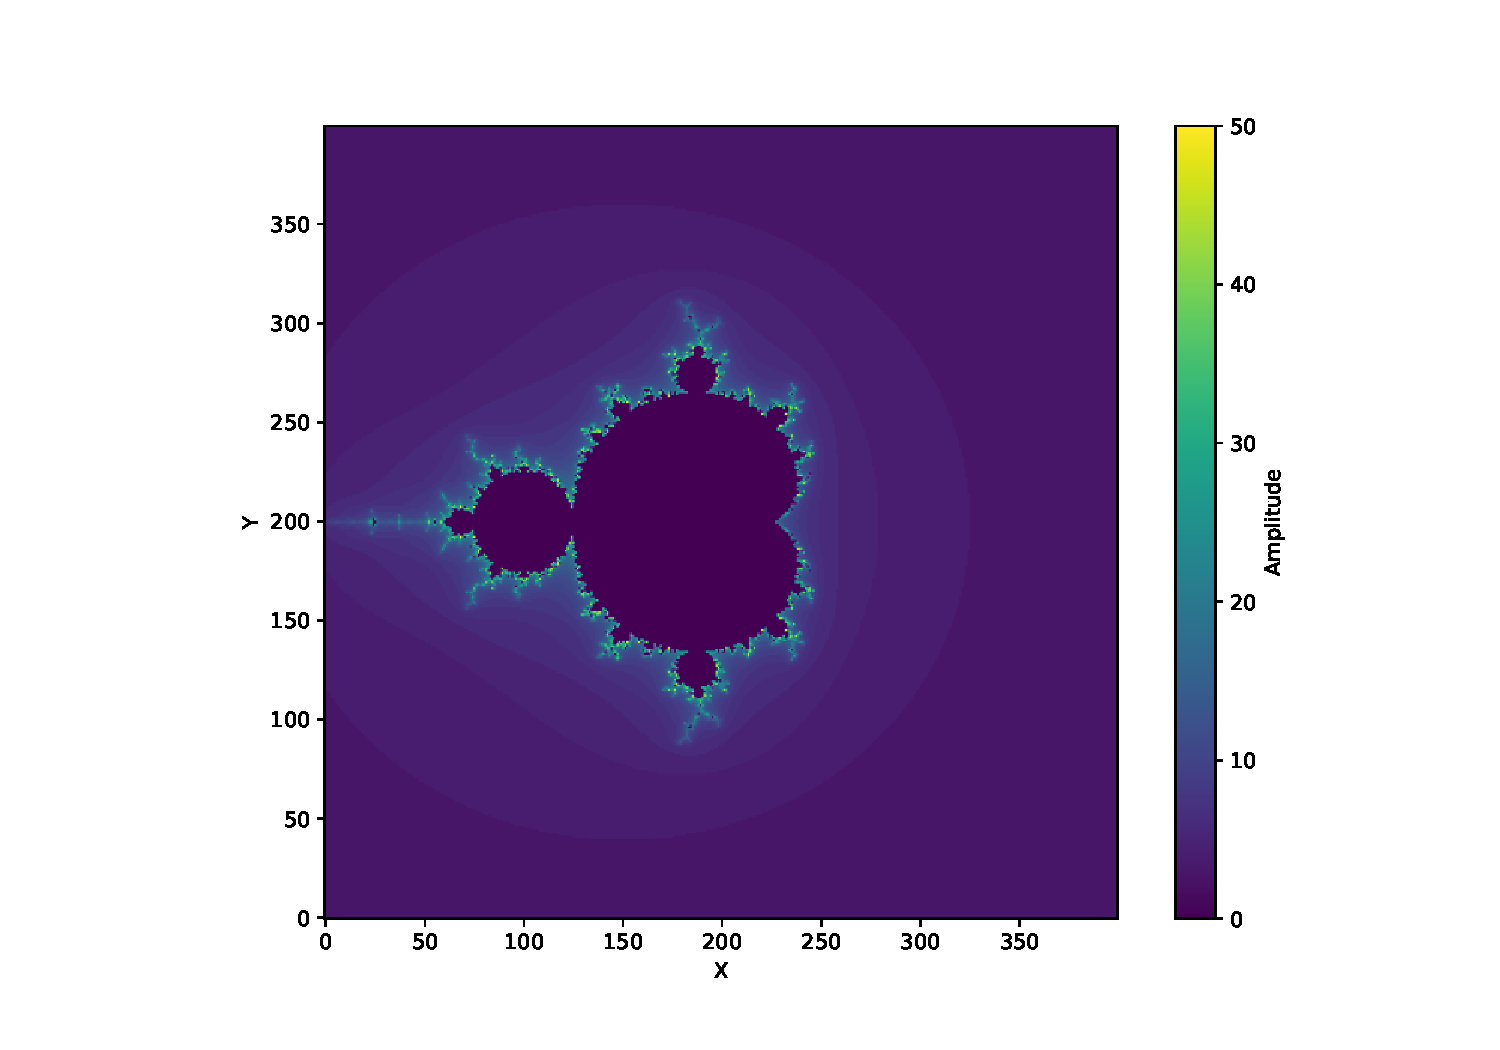
\includegraphics[width =\textwidth]{mandel2.pdf}
        %\vspace{-15mm}
        \caption{The plot of the diverging points colour coded by the iteration step at which a given point will diverge, when iterated through equation \ref{eq:1}. If a point does not diverge, its characteristic number is set to zero.}
        \label{fig:m2}
\end{figure}

\section{Question 2}

Given the following system of differential equations:

\begin{align}
    \dot{X} =& \; -\sigma \left( X - Y \right) \label{eq:2}\\[2mm]
    \dot{Y} =&\; rX - Y - XZ \label{eq:3}\\[2mm]
    \dot{Z} =&\; -bZ + XY \label{eq:4}
\end{align}

discussed in Edward Lorenz's original paper, we may recreate his argument for a chaotic system. We will show that very minute changes in the initial conditions of a system may result in large effects after a given evolution period for the system.

Firstly, we run this system of equations in scipy's ivp solver \textbf{solve\_ivp}, with the initial conditions of $\left( X, Y, Z \right)_0 = W_0 = (0, 1, 0)$, over a period of $60$ units of time. The chosen time step is $\Delta t = 0.01$.

\begin{figure}[H]
    \hspace*{-5mm}
        \centering
        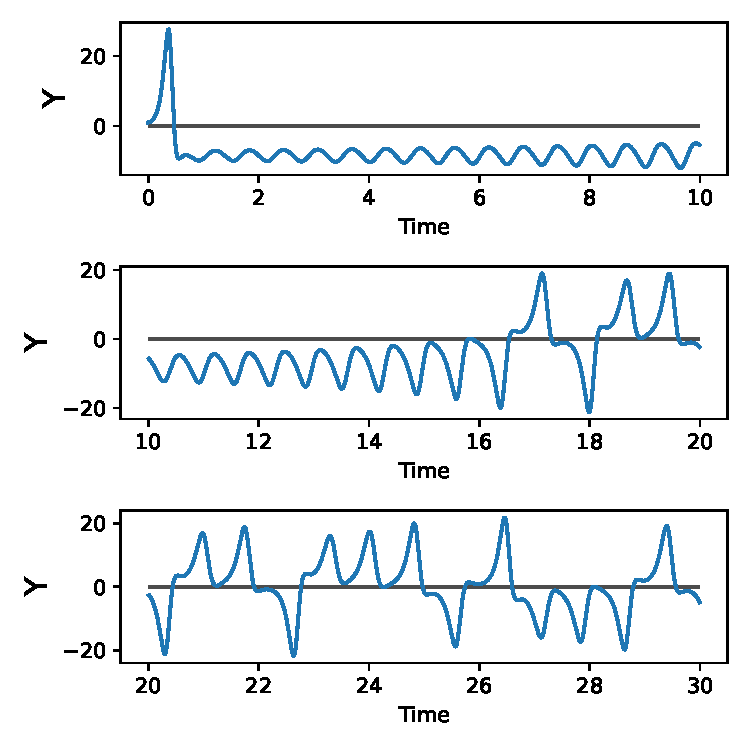
\includegraphics[width =0.5\textwidth]{y_time.pdf}
        %\vspace{-15mm}
        \caption{The solution of $Y$ as a function of time, for the first $30$ units of time. The solution is obtained by the evolution of the system through equations \ref{eq:2}, \ref{eq:3} and \ref{eq:4}.}
        \label{fig:y1}
\end{figure}

We can observe the solution to $Y$ in Figure \ref{fig:y1}, cycling through a few patterns and switching unpredictably from one to the other.

Now plotting the solution $Z$ against $Y$, as well as $X$ against $Y$ in Figure \ref{fig:y2}, we can observe the shape of a `double attractor' forming.
\begin{figure}[H]
    \hspace*{-5mm}
        \centering
        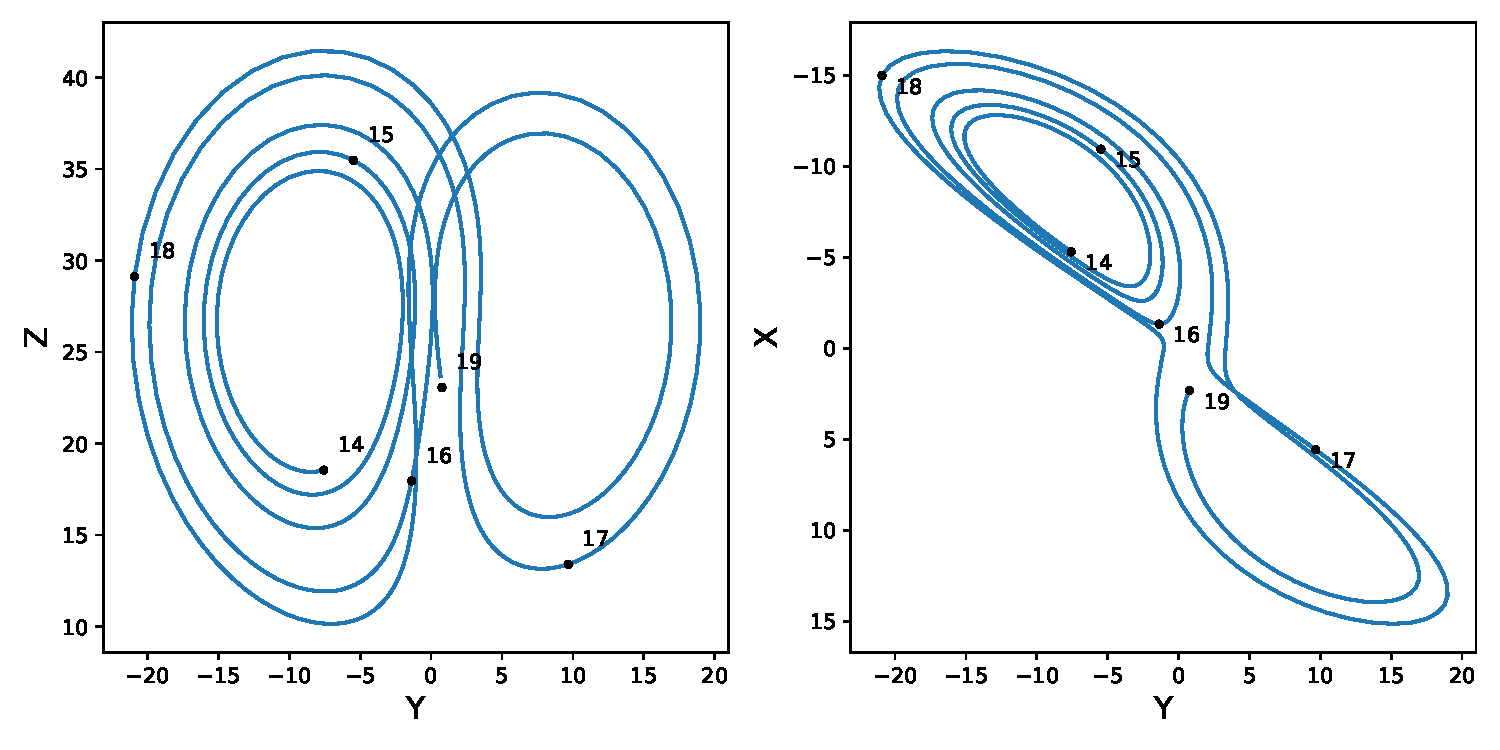
\includegraphics[width =\textwidth]{attract.pdf}
        %\vspace{-15mm}
        \caption{(a) Left: The solution of $Z$ as a function of time, plotted against $Y$ in between $14$ and $19$ units of time. The solution is obtained by the evolution of the system through equations \ref{eq:2}, \ref{eq:3} and \ref{eq:4}. (b) Right: The solution of $X$ as a function of time, plotted against $Y$ in between $14$ and $19$ units of time. The solution is obtained by the evolution of the system through equations \ref{eq:2}, \ref{eq:3} and \ref{eq:4}. The black dots indicate the position of the solution at an indicated instance of time.}
        \label{fig:y2}
\end{figure}

In order to visualize the chaotic effect mentioned above, we may solve the same initial value problem and introduce a small perturbation in the initial condition: $W'_0 = W_0 + (0, 1.e-8, 0)$. Then, we can analyse the distance between $W$ and $W'$ (Euclidian distance between two vectors evolving in time). So, evolving our system again with the new initial conditions and contrasting to the first set of conditions, we can see in Figure \ref{fig:y3} that this distance increases exponentially.

\begin{figure}[H]
    \hspace*{-5mm}
        \centering
        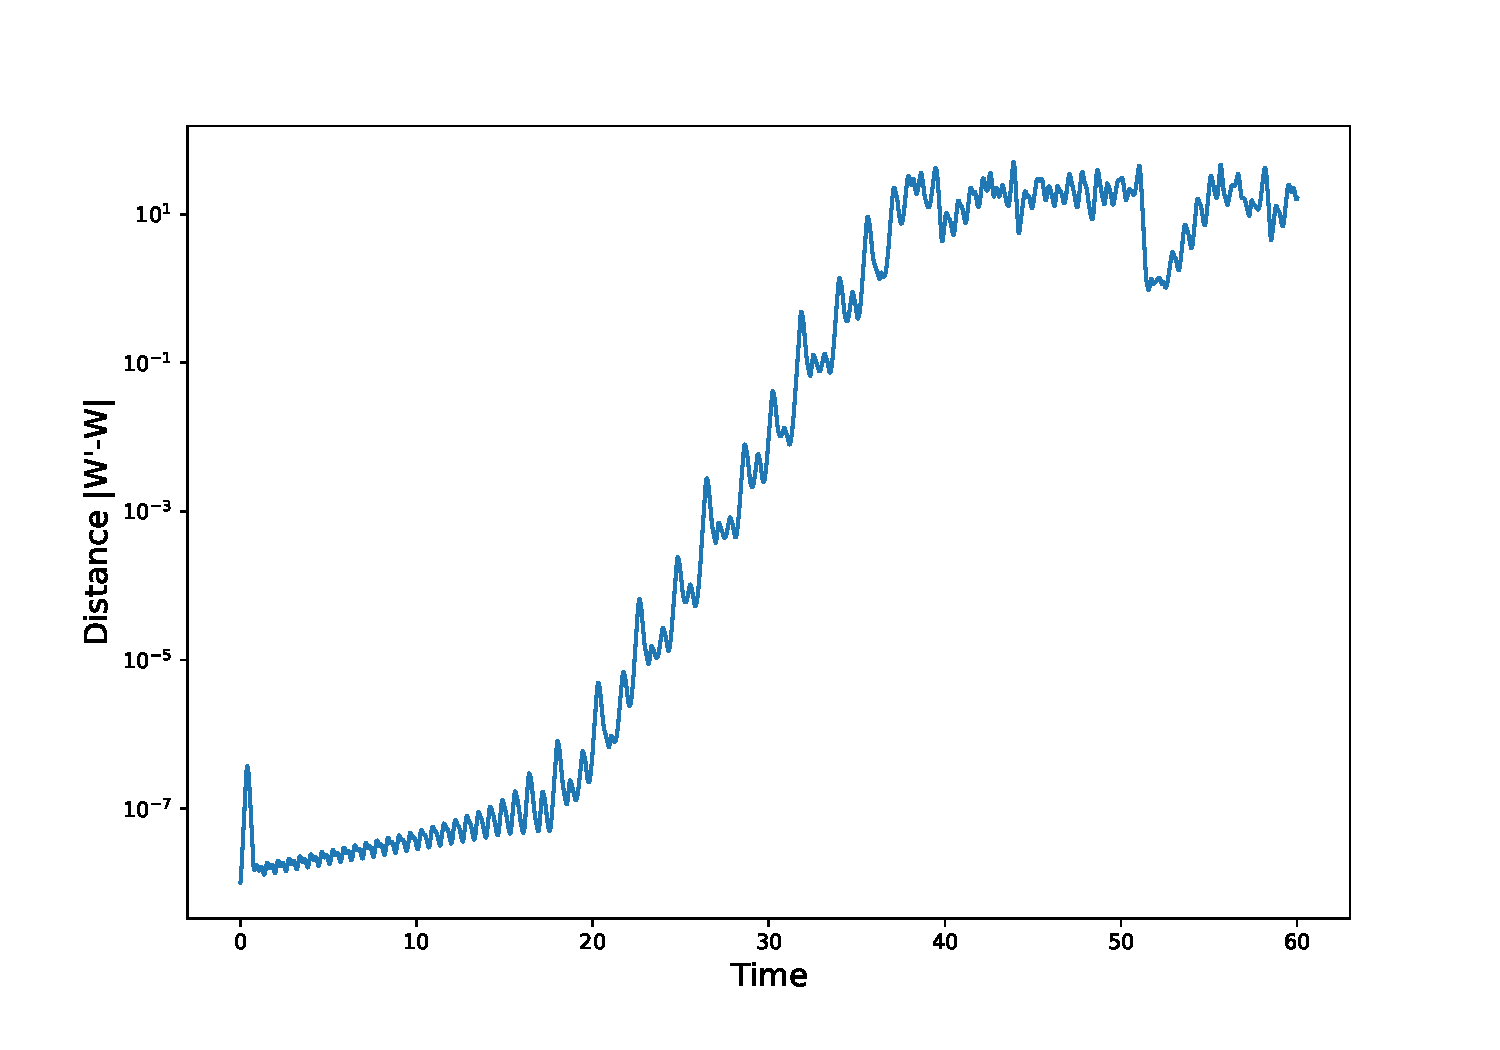
\includegraphics[width =\textwidth]{dist.pdf}
        %\vspace{-15mm}
        \caption{The Euclidian distance between the vectors $W$ and $W'$, defined by the three Lorenz nodes. The solutions of which are found by the evolution of the system through equations \ref{eq:2}, \ref{eq:3} and \ref{eq:4}, with given initial conditions.}
        \label{fig:y3}
\end{figure}

A small perturbation in the initial conditions of the system cause an exponentially differing solution to the first, showing that our system is chaotic and hypersensitive to its initial values.

\end{document}
